\subsubsection{Interface Mémoire}

Le module de mémoire a été conçu de manière générique à l'aide d'interfaces java. Pour cela elle se décompose en trois parties :

\begin{itemize}
\item l'interface principale de la mémoire, qui déclare les méthodes appelées par les autres modules (Analyse et Raisonnement), et qui est implémentée en tant que mémoire à court terme (ActiveMemory),

\item l'interface de la mémoire épisodique et l'interface de la mémoire sémantique, qui déclarent les méthodes appelées par le module Mémoire.
\end{itemize}

\begin{figure}[H]
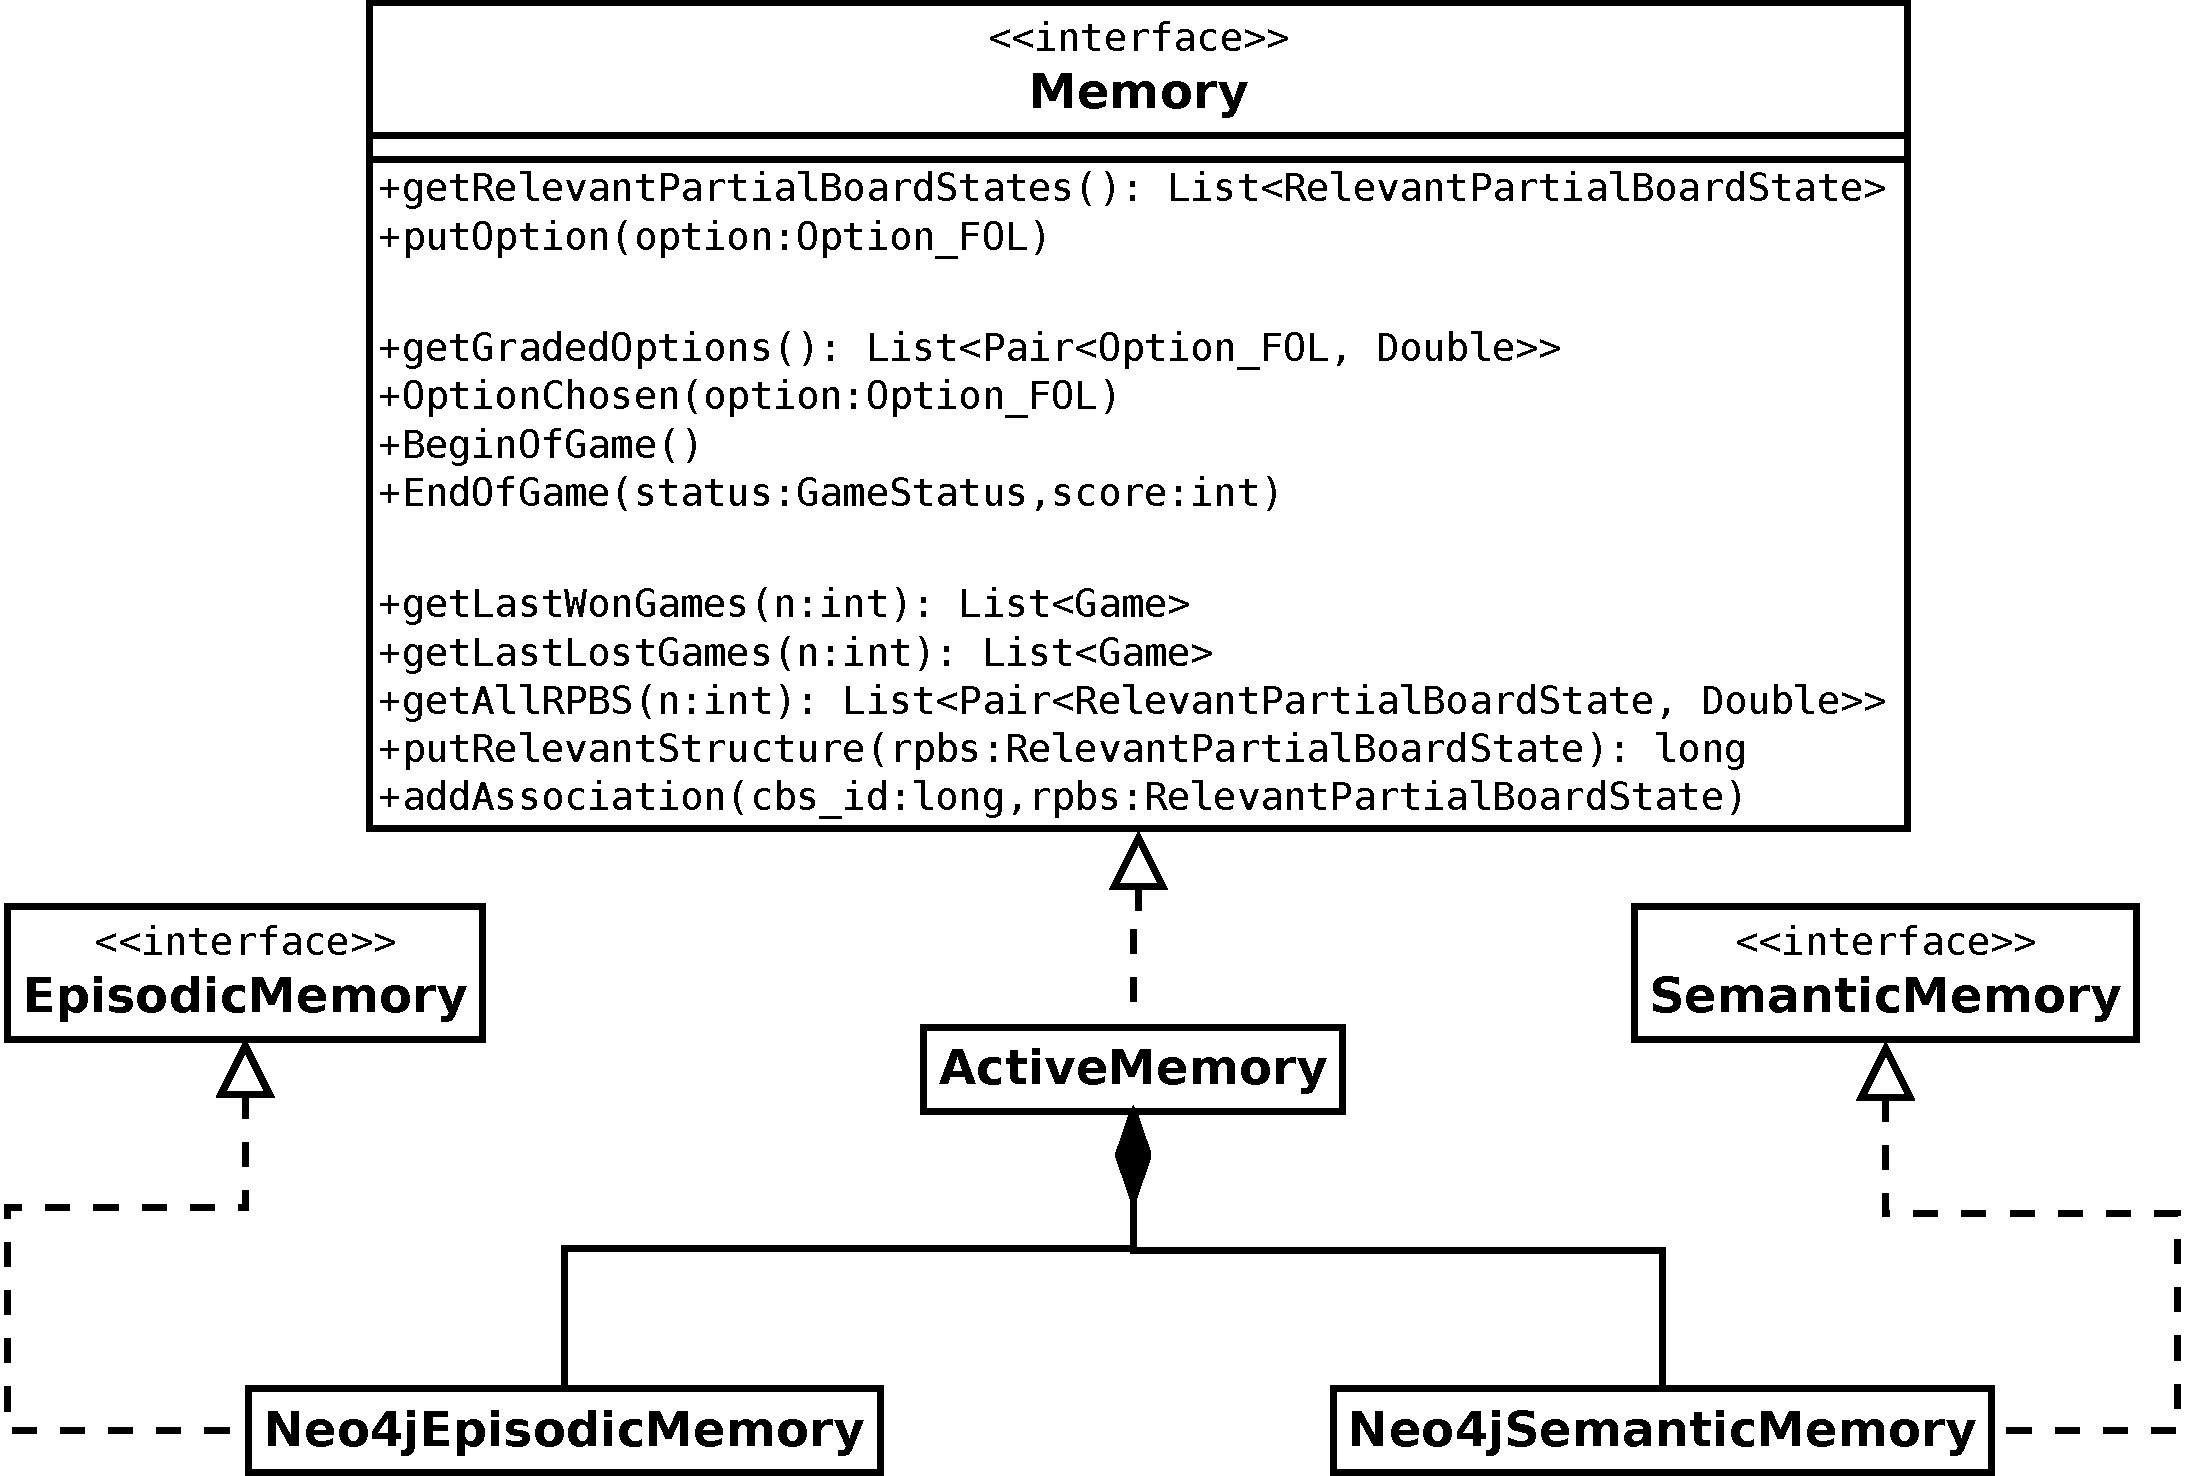
\includegraphics[width=\textwidth]{files/memoire/interface}
\caption{Interface mémoire}
\end{figure}

La mémoire doit également assurer la persistance des données, qui se fait via un module de persistance. Celui-ci est utilisé par une implémentation spécifique des interfaces décrites ci-avant.

\subsubsection{Le SGBD Neo4j}

La persistance des données est assurée par un SGBD né de la mouvance \gls{NoSQL} : Neo4j. Il permet la gestion d'une base de données orientée graphe. Nous avons fait le choix d'utiliser un tel système pour plusieurs raisons :

\begin{itemize}
\item nous avions la volonté de découvrir une solution \gls{NoSQL}, que nous n'avons pas eu l'occasion d'étudier lors de notre formation,

\item Neo4j est disponible en plusieurs versions, notamment en version serveur, version webservice REST et version java embarquée. La mémoire n'étant pas accédée de manière concurrente ainsi que pour des soucis de légèreté, c'est la version embarquée (\emph{embedded java})qui a été utilisée,

\item ce type de SGBD \gls{NoSQL} permet d'obtenir des temps d'accès plus rapides qu'avec des SGBD relationnels traditionnels,

\item la vision graphe de la base de données est adaptée à la conception de notre mémoire\footnote{Notons tout de même qu'il aurait était été possible de stocker les données sous forme de tables},

\item cette solution conserve les propriétés ACID des transactions des SGBD relationnels traditionnels,

\item la documentation complète et la communauté active permettent de s'initier très rapidement à cette nouvelle technologie,

\item Neo4j est une solution libre distribuée sous licence GPLv3.
\end{itemize}

\subsubsection{Mémoire épisodique}

Etiam consequat, ante eget pellentesque placerat, lacus nisl facilisis lectus, nec luctus risus justo quis orci. Sed porttitor, neque quis ullamcorper venenatis, est augue convallis nisi, eu accumsan tortor magna nec urna. Aliquam erat volutpat. Nullam eget nulla nisl. Phasellus porta turpis id mauris eleifend rutrum. Suspendisse varius rhoncus magna, ut commodo ante lacinia at. Nullam viverra malesuada sapien eu luctus. 

\subsubsection{Mémoire sémantique}

Class aptent taciti sociosqu ad litora torquent per conubia nostra, per inceptos himenaeos. Vestibulum arcu massa, hendrerit vel tempor in, sollicitudin in erat. Curabitur non risus nec elit consectetur faucibus sed sed purus. Nam blandit porta ipsum vitae vestibulum. Etiam imperdiet, orci sit amet tincidunt faucibus, urna diam porttitor mauris, at auctor metus neque at nibh. Morbi vel elit venenatis mauris rutrum vehicula. Nam scelerisque iaculis suscipit. Quisque pretium euismod ipsum at elementum. Vestibulum sit amet elit fringilla mauris cursus tincidunt eget sed ante. Ut laoreet ultricies lacus, sed aliquam enim rhoncus ut. Aliquam erat volutpat. Donec ac nulla massa. Maecenas laoreet, magna sed congue venenatis, lacus mi luctus elit, sed sagittis justo nisi ut felis. Aliquam interdum, leo non vestibulum euismod, enim eros eleifend ligula, at aliquet mi eros vitae diam. Suspendisse malesuada scelerisque quam at sodales. Fusce ac lacus sed massa pretium bibendum. 

\subsubsection{Gestion de la persistance}

Ut tincidunt blandit venenatis. Praesent vel nibh vel sem viverra eleifend a rhoncus dolor. Praesent vestibulum orci mattis tellus sagittis sit amet sollicitudin elit gravida. Nam dapibus luctus tortor, ut sodales enim ultrices vel. Nulla urna urna, elementum vehicula porta ut, varius ut turpis. Vestibulum iaculis dolor sed est tempus nec imperdiet massa mollis. Ut in dignissim felis. Cras aliquet, turpis vel fermentum sollicitudin, elit
nulla

lobortis neque, ut tristique justo metus quis urna. Integer tincidunt, dolor ac sodales venenatis, metus dui bibendum mi, nec vehicula est neque volutpat libero. Nunc viverra rhoncus neque nec ultricies. Praesent consectetur metus et mi placerat ac fringilla sem congue. Nullam eu nisl in arcu condimentum fringilla. 

Ut tincidunt blandit venenatis. Praesent vel nibh vel sem viverra eleifend a rhoncus dolor. Praesent vestibulum orci mattis tellus sagittis sit amet sollicitudin elit gravida. Nam dapibus luctus tortor, ut sodales enim ultrices vel. Nulla urna urna, elementum vehicula porta ut, varius ut turpis. Vestibulum iaculis dolor sed est tempus nec imperdiet massa mollis. Ut in dignissim felis. Cras aliquet, turpis vel fermentum sollicitudin, elit nulla lobortis neque, ut tristique justo metus quis urna. Integer tincidunt, dolor ac sodales venenatis, metus dui bibendum mi, nec vehicula est neque volutpat libero. Nunc viverra rhoncus neque nec ultricies. Praesent consectetur metus et mi placerat ac fringilla sem congue. Nullam eu nisl in arcu condimentum fringilla. 
